\documentclass[CS4204-Notes.tex]{subfiles}
\begin{document}

\section{Parallel patterns}
A \textbf{pattern} is a common way of introducing parallelism which helps with the program design and helps to guide the implementation. Often a pattern may have several different implementations, for example a \textit{map} can be implemented as a \textit{task farm}. Different implementations may then have different performance characteristics. There are primarily two forms of underlying parallelism: \textbf{data parallelism} and \textbf{task parallelism}.
\begin{figure}[H]
\centering
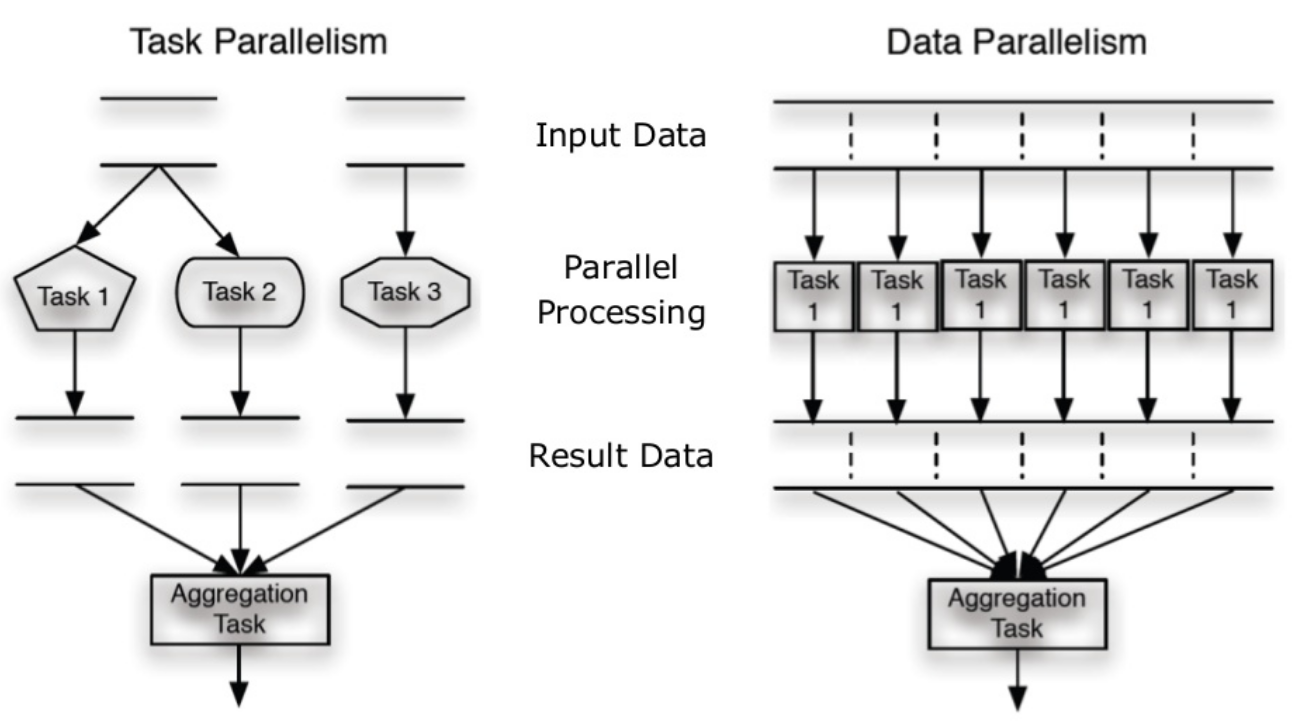
\includegraphics[width=0.7\textwidth, keepaspectratio]{imgs/task-data-parallelism.png}
\caption{Difference between task and data parallelism.}
\end{figure}

\subsection{Data parallelism}
Data parallelism comes from parallelism that is primarily extracted from the structure of the data that operations are applied to. Operations are applied \textit{independently} to several data items, for example the same operation to all elements of a list or array. Data parallelism is generally more regular (that is to say all parallel tasks have similar sizes and functionality) and involves less complex programming structures. Typically data-parallelism may produce large amounts of very fine-grained parallelism which is a good fit for massively parallel architectures like GPUs or SIMD vector architectures. 
\n
Examples of data parallel patterns include:
\begin{itemize}
\item Parallel maps
\item Parallel scans
\item Map-reduce
\end{itemize}

\subsection{Task parallelism}
In contrast to data parallelism, task parallelism comes from the control flow in a program. This is more flexibly than data-parallelism but often exposes less parallelism and is harder to conceptualise. Further, task-parallelism has a less regular size and structure, as each part of the control flow can have different functionality, making it difficult to manage at runtime. 
\n
Examples of task parallel patterns include:
\begin{itemize}
\item Piplines
\item Divide and conquer
\item Task farm
\end{itemize}

\subsection{Data parallel patterns}
\subsubsection{Parallel maps}
Parallel maps are one of the simplest forms of data parallelism and is also one of the most useful. Sequential maps are very commonly used in sequential Haskell to apply a function to every element in a list. Parallelising this simply involves applying the function in parallel to every element, creating extra threads to evaluate parts of the list. 
\begin{figure}[H]
\centering
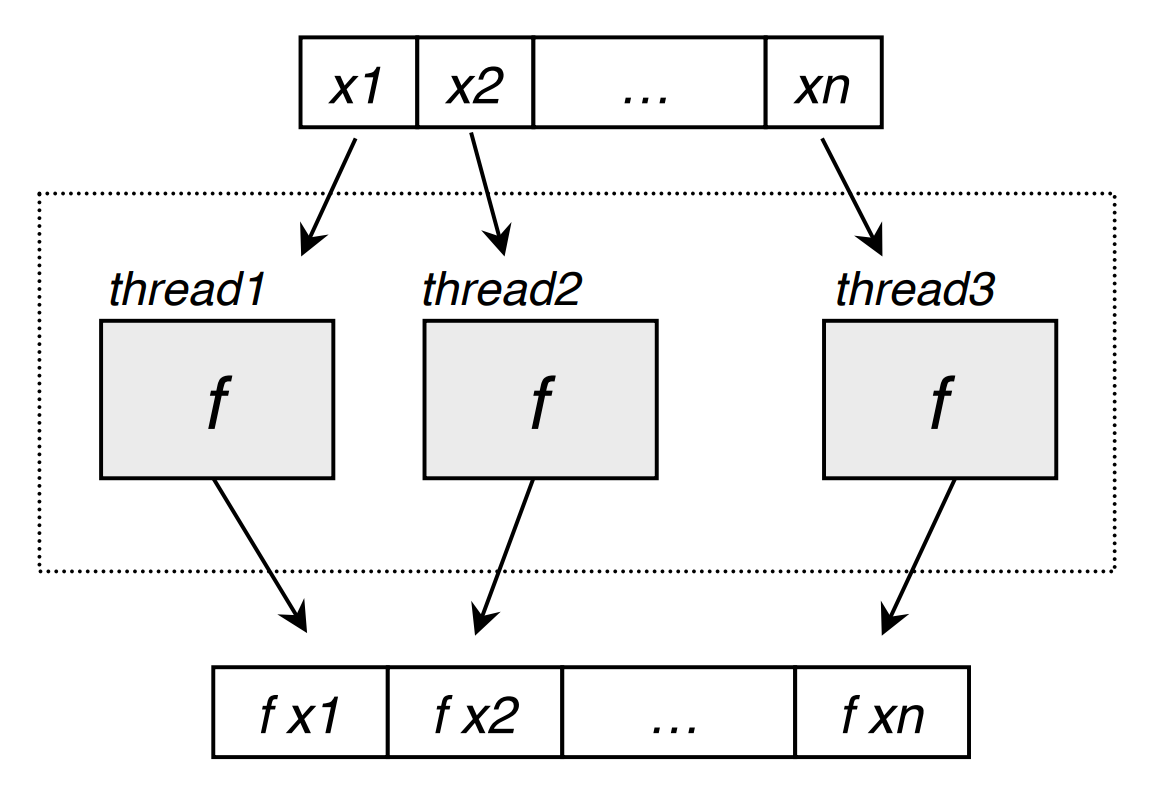
\includegraphics[width=0.5\textwidth, keepaspectratio]{imgs/parallel-map.png}
\caption{Parallel maps map a function across each element in parallel.}
\end{figure}
\noindent

\begin{lstlisting}[caption={Parallel map implementation}]
parmap :: (a -> b) -> [a] -> [b]
parmap f [] = []
parmap f (x:xs) = let fx = f x in
					fx <@\textcolor{red}{\textquoteback par\textquoteback}@> (fx : map f xs)
\end{lstlisting}
\texttt{parmap} can be used anywhere where standard sequential \texttt{map} is used. Although this can be done by simply replace all instances of \texttt{map} with \texttt{parmap}, it may not lead to efficient parallelism. There are a few caveats that need to be taken into account to achieve good parallel performance:
\begin{itemize}
\item All elements of the data structure must already have been evaluated before the \texttt{parmap} is applied
\item There must be no dependencies between the results of the parallel map
\end{itemize}

\subsubsection{Parallel zipWith}
A \texttt{zipWith} is a kind of map that works over two input lists. It maps a function across a pair of elements rather than single elements from one list. The operation \textit{op} is allied in parallel to each pair of elements \textit{x1},\textit{y1} etc. to give the resulting list. The final result is evaluated using a given strategy. As usual, the function calls are only worth evaluating in parallel is the operation \textit{op} is expensive. 
\begin{figure}[H]
\centering
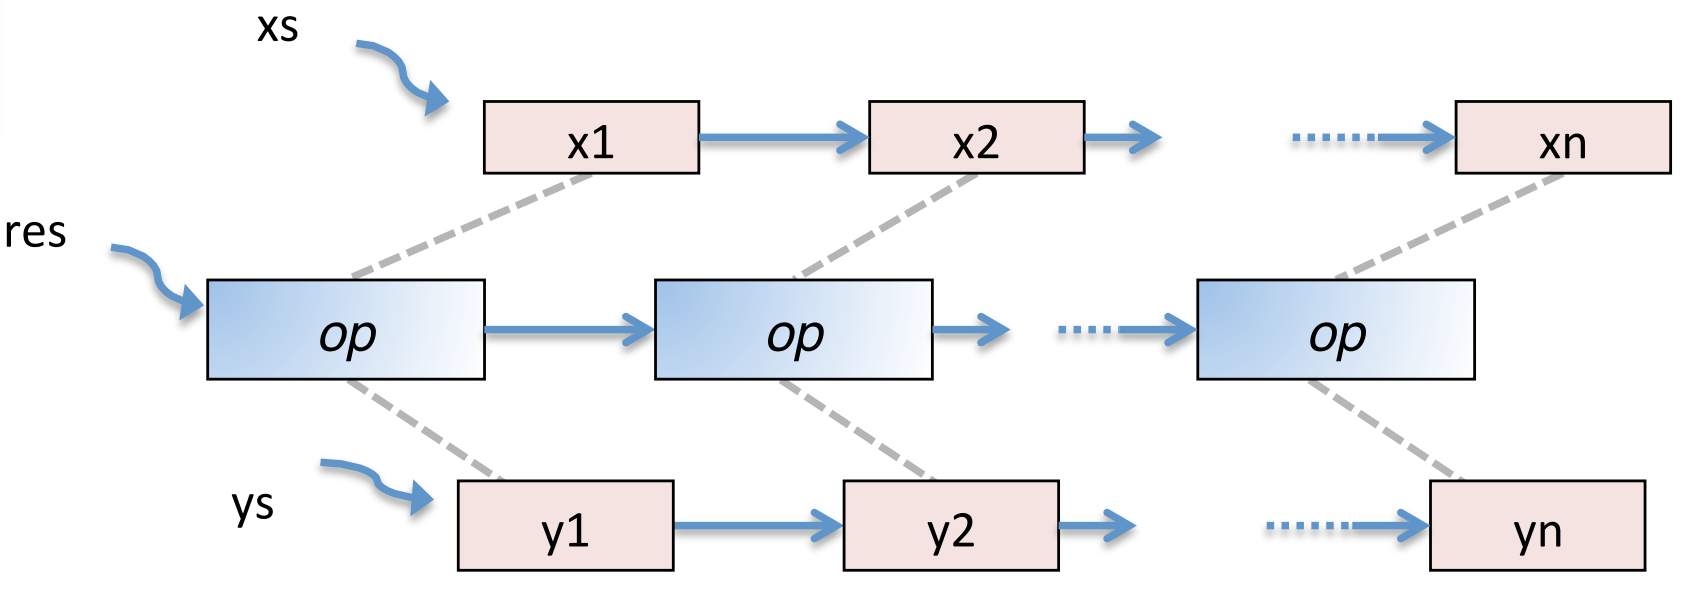
\includegraphics[width=0.9\textwidth, keepaspectratio]{imgs/parallel-zipwith.png}
\caption{Parallel \texttt{zipWith} over two input lists \texttt{xs} and \texttt{ys}}
\end{figure}

\subsubsection{Parallel fold (reduce)}
A fold is a more complex pattern that applies an operator \textit{between} each pair of elements in a list. They can be easily parallelised, however care must be taken over the properties of the operator being used. 
\begin{lstlisting}[caption={Type signature of a parallel fold.}]
parFold :: (a -> a -> a) -> a -> [a] -> a
parFold f z l = ...

-- Examples of fold uses
sum = parFold (+) 0
product = parFold (*) 1
\end{lstlisting}

\begin{figure}[H]
\centering
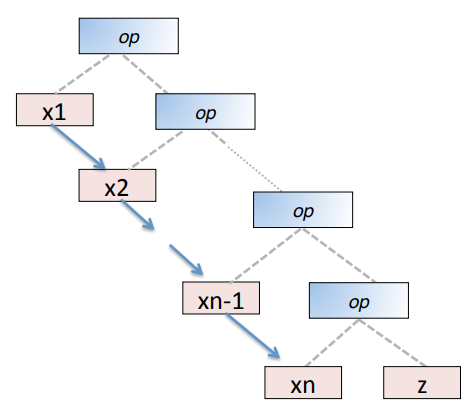
\includegraphics[width=0.5\textwidth, keepaspectratio]{imgs/sequential-fold.png}
\caption{Sequential right fold.}
\end{figure}

\begin{figure}[H]
\centering
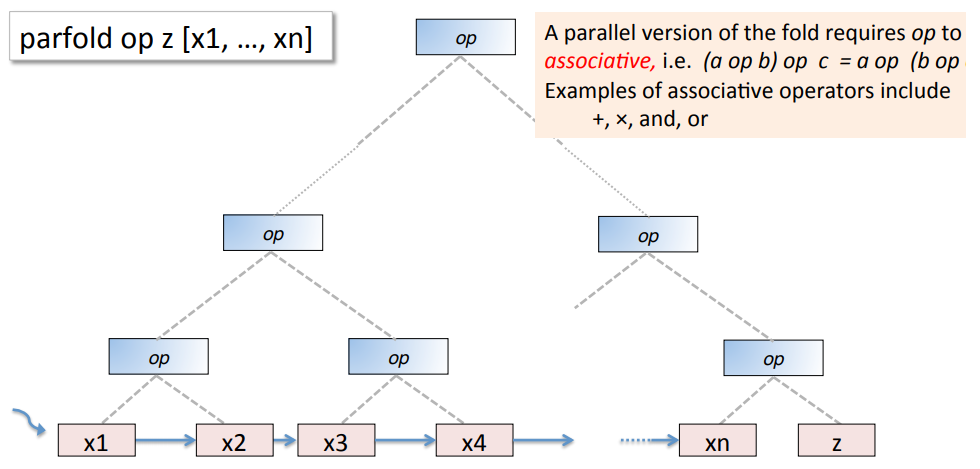
\includegraphics[width=0.9\textwidth, keepaspectratio]{imgs/parallel-fold.png}
\caption{Parallel fold.}
\end{figure}
\noindent
The parallel version of fold requires \textbf{associative} operators because the order of applying the operators cannot matter. This allows the internal computations of the fold to be reordered to give better parallel behaviour. Each operation can be executed by a separate thread and the results combined independently in a tree-like manner. This could not have been done with an associate operator, as the elements of the list cannot be reordered and keep the same result. 

\subsubsection{Bulk Synchronous Parallelism (BSP)}
Bulk synchronous parallelism is a more complicated and sophisticated data-parallel pattern. BSP computations proceeds in a series of \textbf{supersteps} where all threads perform the same computation on different data on each superstep, similar to a parallel map. The difference is that after each superstep, all threads synchronise and exchange some or all data with other threads as needed. The threads are synchronised by barrier, meaning all threads wait until data exchange is completed for all other threads before starting the next superstep. This is potentially very expensive when all other threads are blocked waiting for one or two threads to finish but guarantees that all threads have produced and exchanged information which means no deadlock or livelock. 
\begin{figure}[H]
\centering
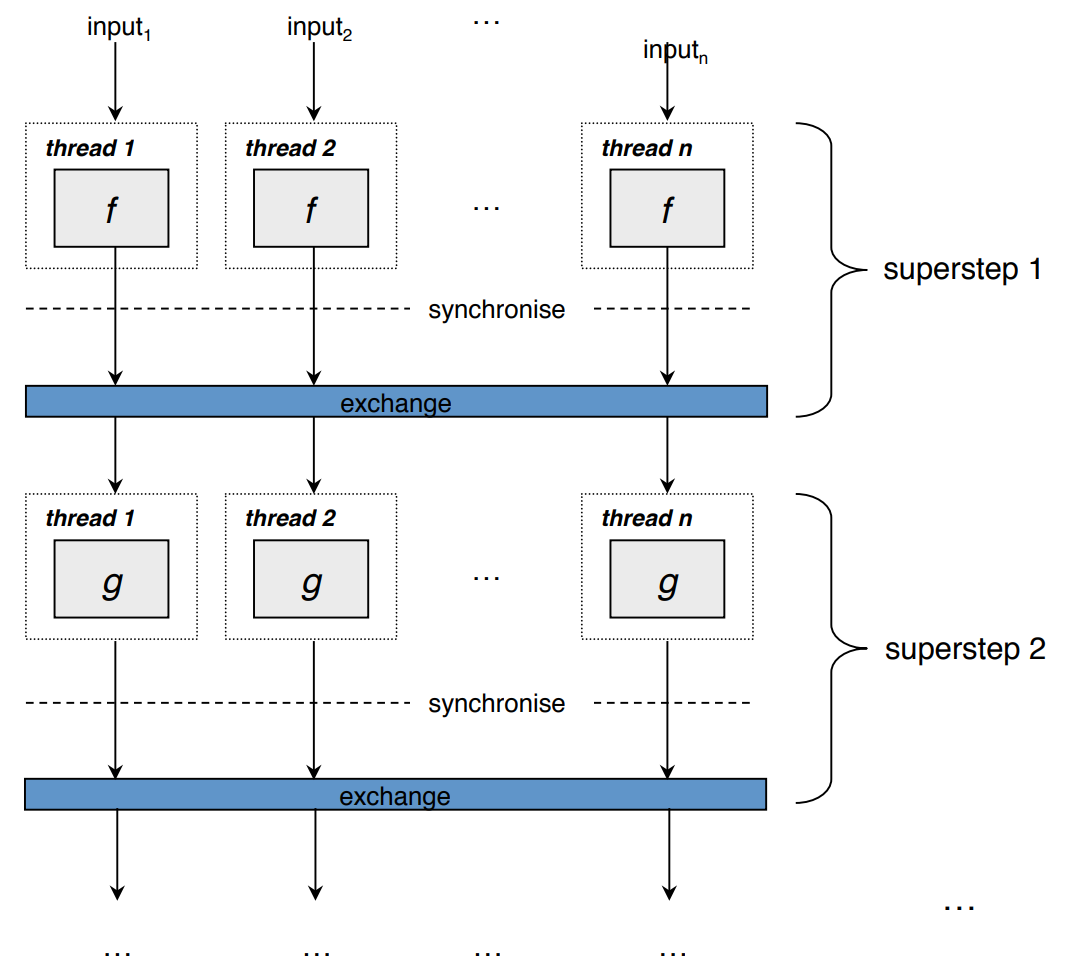
\includegraphics[width=0.6\textwidth, keepaspectratio]{imgs/bsp.png}
\caption{The bulk synchronous parallelism process.}
\end{figure}
\noindent
During each superstep, each thread works on its own inputs using \textit{private local data} and \textit{shared global data}. This global and local data is exchanged between each superstep. The global data from all threads is combined to give a new list of global data, which is then passed as a single value to all of the threads that are evaluating the next worker task. Each thread has its own local state which may be altered as a result of the computation at each superstep. Threads also have access to the global state. During the exchange, each thread produces new local and global state. The global state can only be changed during the exchange. 
\begin{figure}[H]
\centering
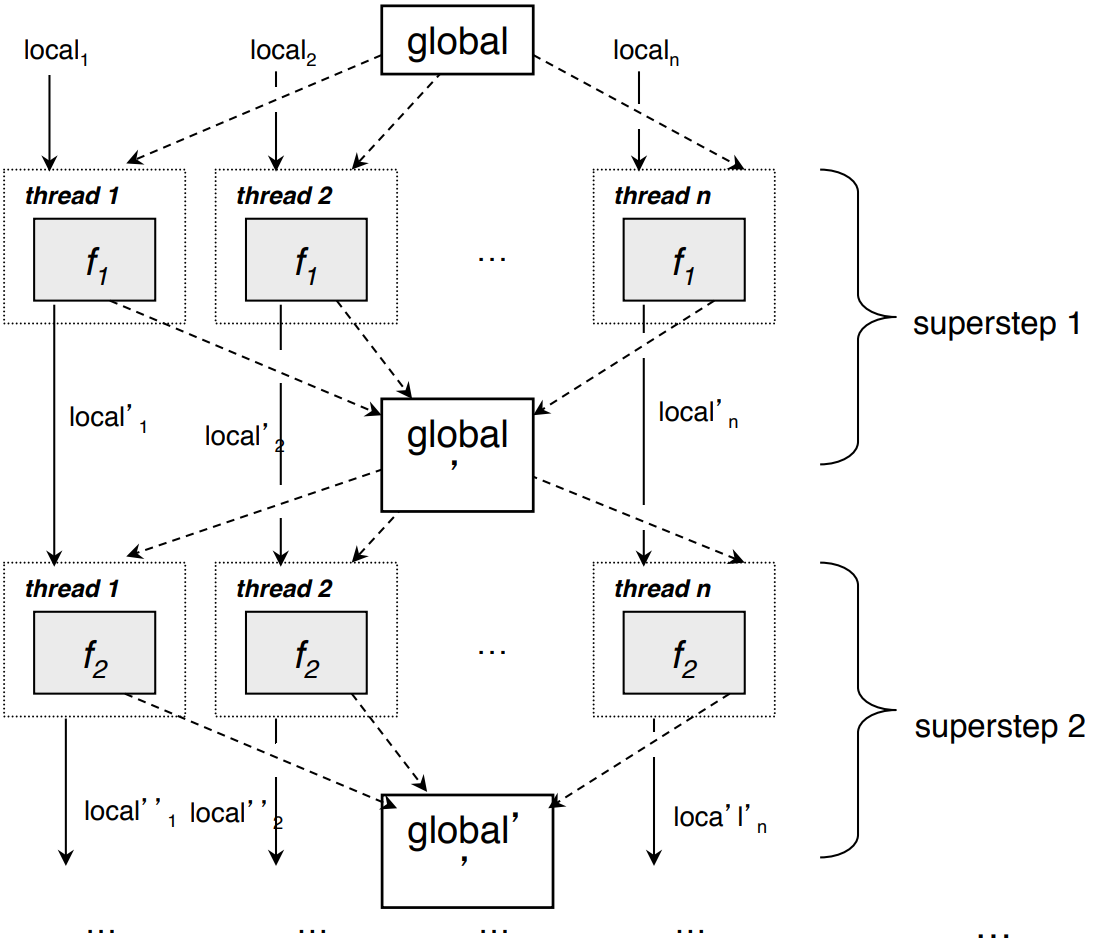
\includegraphics[width=0.6\textwidth, keepaspectratio]{imgs/bsp-exchange.png}
\caption{BSP local and global data exchange process.}
\end{figure}
\noindent
BSP works well when each computation in every superstep has a similar size. The weakness is that in the synchronisation phase, if an operation takes different amounts of time for different inputs, individual threads may be blocked for significant periods of time waiting for other threads to complete. 
\n
The BSP pattern also provides a simple model of parallel execution cost. Since the global synchronisation waits on all threads, the amount of time taken to execute a superstep is always the same for all threads. Further, it follows that the exchange step has the same fixed constant size. This gives the following equation for the time required to execute a complete sequence of $m$ BSP supersteps
\begin{equation}
\sum_{i=1}^{m}f_{i} + c_{ex} \times (m - 1)
\end{equation}
where 
\begin{itemize}
\item $f_{i}$ is the maximum cost of the operation at step $i$
\item $c_{ex}$ is the cost of exchange/synchronisation
\item $m$ is the number of supersteps
\end{itemize}
This calculation assumes that there are enough processors available to execute all of the threads that are created to execute the pattern. 
\subsubsection{Parallel map-reduce}
Map-reduce is a common pattern that has been applied to commercial, large, distributed server farms for dealing with big data. It uses a combination of \textit{map} to map a function across the data and a \textit{reduce} to reduce the results to simpler values. It works by splitting the input into a large number of similarly sized tasks that can be processed independently using the \textit{map} operation. Then each intermediate group of data can be processed with the \textit{reduce} function. 
\begin{figure}[H]
\centering
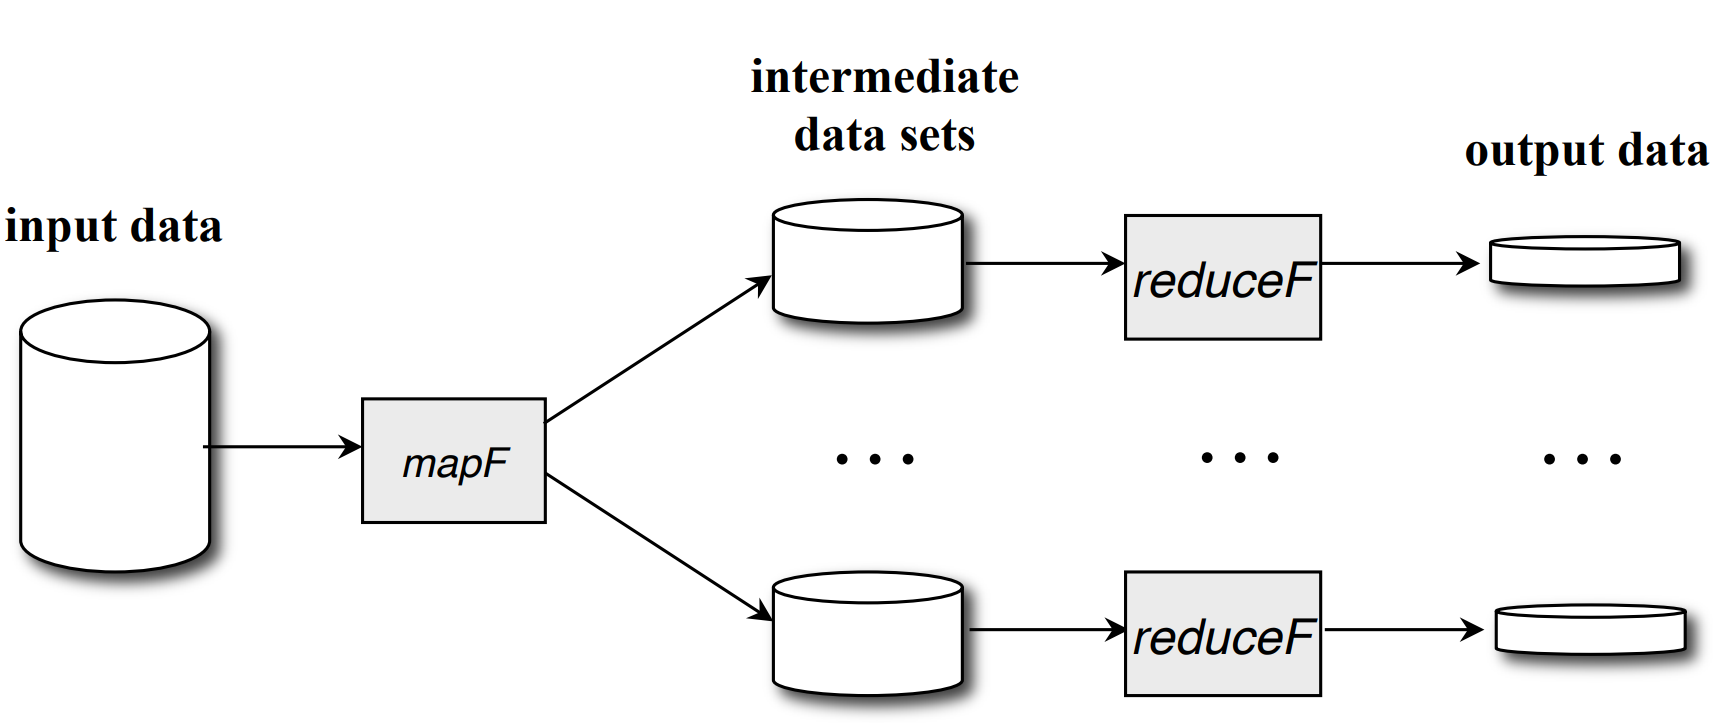
\includegraphics[width=0.9\textwidth, keepaspectratio]{imgs/map-reduce-simple.png}
\caption{Map-reduce with parallel reduction step.}
\end{figure}
\noindent
Quite clearly the reduce operations can be run in parallel with data parallelism, using a parallel map to map the reduce function to the data. However, it is also possible to increase the parallelism by running the map operations in parallel by splitting the data and them mapping each map in parallel. If the reduction operation is associative, each set of intermediate results may then be reduced independently: a local reduce function is applied to each intermediate set of results and an overall reduce function applied at the end of get the final result. 
\begin{figure}[H]
\centering
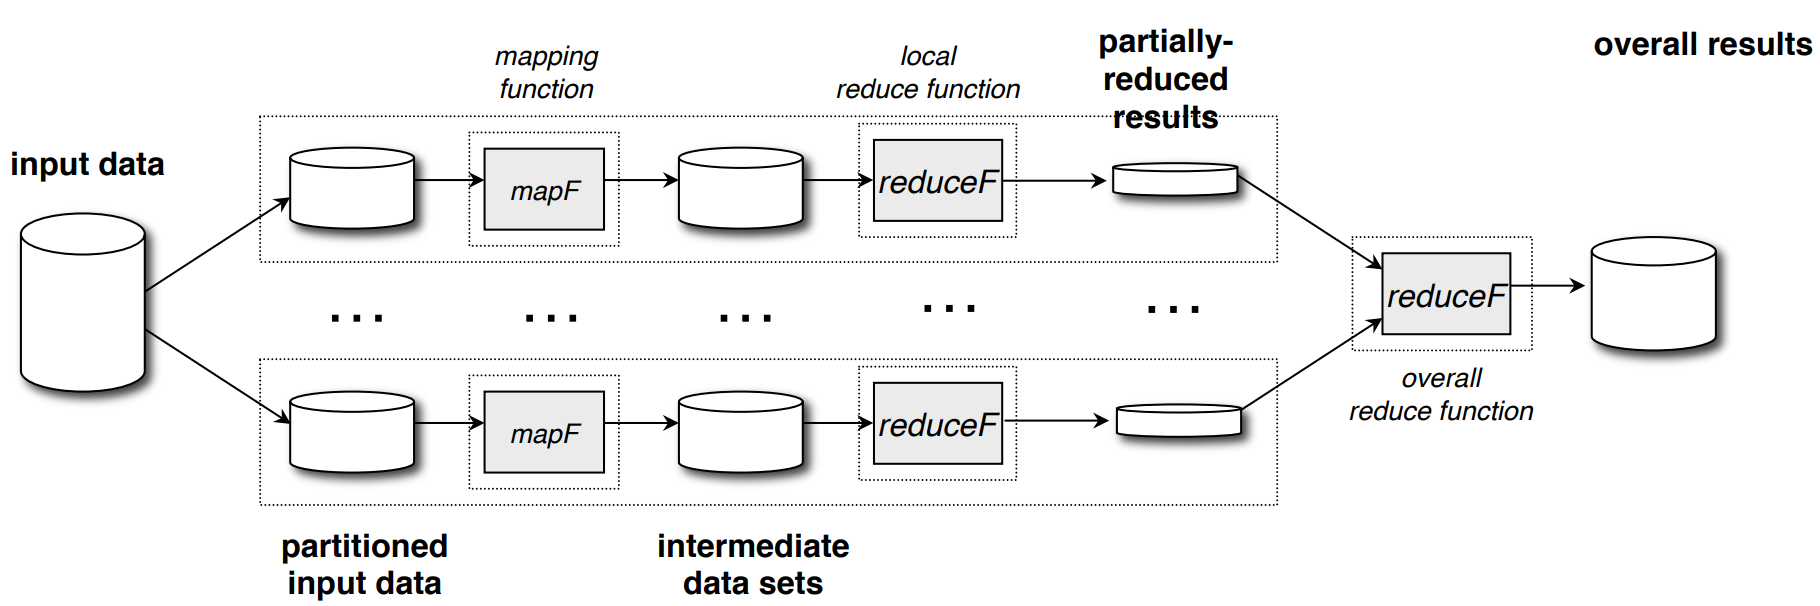
\includegraphics[width=1\textwidth, keepaspectratio]{imgs/map-reduce-more.png}
\caption{Map-reduce with parallel mapping step.}
\end{figure}

\subsubsection{Parallel scan}

\end{document}